% OWD 2026
% HIPC Assessment Presentation

% TODO: CUDA timings for graph
% TODO: CUDA timings breakdowns
% TODO: CUDA roofline plots

\documentclass{beamer}

\usepackage{listings, calc, booktabs, pgfplots}
\usepackage[en-GB]{datetime2}
\usepackage[
    backend=biber,
    style=authoryear,
    citestyle=authoryear,
    bibencoding=utf8
]{biblatex}

\pgfplotsset{compat=1.18}
\definecolor{seriallegend}{RGB}{179,179,255}
\definecolor{openmplegend}{RGB}{255,179,179}
\definecolor{mpilegend}{RGB}{236,217,198}
\definecolor{cudalegend}{RGB}{128,128,128}

\addbibresource{references.bib}
\usetheme{CambridgeUS}
\setbeamertemplate{caption}[numbered]
\numberwithin{figure}{section}
\beamerdefaultoverlayspecification{<+->}
\setbeamertemplate{navigation symbols}{}

\hypersetup{
    colorlinks,
    allcolors=.,
    urlcolor=gray,
}

\definecolor{codegreen}{rgb}{0,0.6,0}
\definecolor{codegray}{rgb}{0.5,0.5,0.5}

\lstdefinestyle{mystyle}{
    otherkeywords={compute\_t,\#pragma,schedule,nowait,collapse,indexer\_t},
    columns=fullflexible,
    commentstyle=\color{codegreen},
    keywordstyle=\color{magenta},
    numberstyle=\tiny\color{codegray},
    basicstyle=\ttfamily\tiny,
    breakatwhitespace=false,
    breaklines=true,
    captionpos=b,
    keepspaces=true,
    showspaces=false,
    showstringspaces=false,
    showtabs=false,
    tabsize=2
}

\lstset{style=mystyle}

\title{Review of Parallelised CFD Solvers}
\date{\today}
\author[Oliver Dixon]{
    \texorpdfstring{Oliver Dixon \raisebox{.5pt}{%
        \texttt{\footnotesize\href{mailto:Oliver Dixon <od641@york.ac.uk>}
            {<od641@york.ac.uk>}}
    }}{Oliver Dixon}}
\institute[University of York]{Department of Computer Science, University of York}
\subtitle{HIPC-H Assignment Presentation}

\begin{document}
\frame{\titlepage}
\section{Optimisation and Parallelisation Approach}
\begin{frame}
    \frametitle{Analysis of the Serial Implementation}
    \begin{itemize}
        \item The serial implementation provides a validated baseline for
            iterative computation of velocity vectors and pressure scalars
            around a rigid body specified as a NACA airfoil.
        \item For successive time-steps, the solver executes a series of
            sub-routines to numerically improve upon the simulation state:
            \begin{enumerate}
                \item Apply \emph{no-slip} boundary conditions;
                \item Compute tentative velocities;
                \item Compute the forcing term for the Poisson equation;
                \item Iteratively solve the Poisson PDE to provide pressure
                    scalars;
                \item Update velocity estimates according to tentative values
                    and neighbouring pressures.
            \end{enumerate}
        \item This is a standard approach in CFD applications and most of these
            sub-routines are \emph{embarrassingly
            parallel}\footfullcite{Griebel:1998}.
    \end{itemize}
\end{frame}
\begin{frame}
    \frametitle{OpenMP Implementation Strategy (1)}
    \begin{itemize}
        \item On-node parallelism has no significant implementation-level
            deviations from the serial equivalent.
        \item Efforts primarily aimed at Red-Black SOR routine.
            \begin{itemize}
                \item Analysis with the \emph{Intel Advisor} indicated that the
                    OneAPI compiler could not vectorise the NAST2D
                    implementation.
                \item Minimised branching and packed neighbouring values into
                    arrays to encourage usage of AVX2 registers.
                \item Existing use of red-black colouring scheme reduces natural
                    data dependencies \footfullcite{Sparsh:2014}.
            \end{itemize}
        \item Where the \emph{Advisor} and \emph{VTune} suggested advantageous,
            OpenMP with static loop-scheduling and collapsing was used.
        \item Where there were no data dependencies between parallel regions,
            asynchronous OMP was used to eliminate implicit barriers.
    \end{itemize}
\end{frame}
\begin{frame}
    \frametitle{OpenMP Implementation Strategy (2)}
    \begin{center}
        \begin{minipage}{.7\textwidth}
            \lstinputlisting[language=C]{code-samples/omp-async-loop.c}
        \end{minipage}

        Dependency-Free Loop Pair with Asynchronous OMP Parallel Regions

        \footnotesize\texttt{openmp/region.c:region\_update\_velocities}
    \end{center}
\end{frame}
\begin{frame}
    \frametitle{MPI Implementation Strategy (1)}
    \begin{itemize}
        \item Two-dimensional domain decomposition into roughly equally sized
            portions, each allocated to a rank
            process\footfullcite{Griebel:1998}.
            \begin{itemize}
                \item Automatic computation of subdomain boundaries at runtime
                \item Subdomains `overlap' to provide ghost rows and columns
                \item Ghost cells are populated with extremities of neighbouring
                    regions, achieved with halo exchanges
                \item Subdomains are marked with flags dependent on their
                    position within the virtual Cartesian topology
            \end{itemize}
        \item Non-blocking communication used where possible; barriers enforced
            with explicit blocking calls provided by OpenMPI.
    \end{itemize}
\end{frame}
\begin{frame}
    \frametitle{MPI Implementation Strategy (2)}
    \begin{center}
        \begin{minipage}{.85\textwidth}
            \lstinputlisting[language=C]{code-samples/mpi-maximise.c}
        \end{minipage}\vfill%
        Maximising velocities across ranks

        \footnotesize\texttt{mpi/region.c:region\_update\_timestep\_interval}
    \end{center}
\end{frame}
\begin{frame}
    \frametitle{CUDA Implementation Strategy (1)}
    \begin{itemize}
        \item Domain decomposition not explicit as in MPI, but requires careful
            mapping to ensure memory coalescing.
            \begin{itemize}
                \item One-dimensional arrays mapped into a column-major ordering
                    to index at constant stride offsets.
                \item Host and device memory explicitly aligned on word/TB
                    boundaries with \texttt{\_\_align\_\_}.
            \end{itemize}
        \item Halo exchanges not required, and reductions occur in shared
            memory with explicit block-level synchronisation provided by
            \texttt{\_\_syncthreads}\footfullcite{Harris:2007}. 
        \item CUDA provides runtime API to dynamically choose optimum block
            size, based on GPU topology and problem size, with
            \texttt{cudaOccupancyMaxPotentialBlockSize}.
    \end{itemize}
\end{frame}
\begin{frame}
    \frametitle{CUDA Implementation Strategy (2)}
    \begin{center}
        \begin{minipage}{.85\textwidth}
            \lstinputlisting[language=C]{code-samples/cuda-reduction.cu}
        \end{minipage}\vfill%
        Shared-memory reduction across thread blocks

        \footnotesize\texttt{cuda/DeviceRegion.cu:kernels::reduce\_sum\_kernel<class T>}
    \end{center}
\end{frame}
\begin{frame}
    \frametitle{Validation of Correctness (1)}
    \begin{itemize}
        \item In all ports, a VTK serialiser was implemented to produce vector
            and scalar vector fields viewable in \emph{LLNL VisIt}.
        \item OpenMPI and CUDA collect the entirety of the data-set onto a
            single host thread following computation and serialises into a
            single XML VTR (VTK rectangle) ASCII file.
        \item MPI uses VTR-P files to distribute results into separate files,
            each written by their respective node, which are collated by a
            metadata file produced by the master rank\footfullcite{VTK:2021}.
            \begin{itemize}
                \item Avoids complexity of MPI file-handling routines.
                \item Supported by all major implementations of the VTK format.
            \end{itemize}
    \end{itemize}
\end{frame}
\begin{frame}
    \frametitle{Validation of Correctness (2)}
    \begin{figure}
        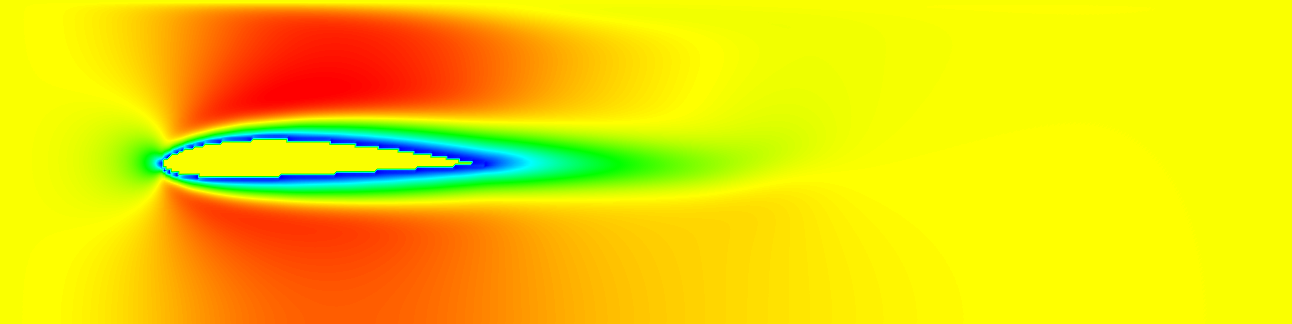
\includegraphics[width=.8\linewidth]{output/velocities}
        \caption{Velocity Magnitudes}
    \end{figure}
    \pause%
    \begin{figure}
        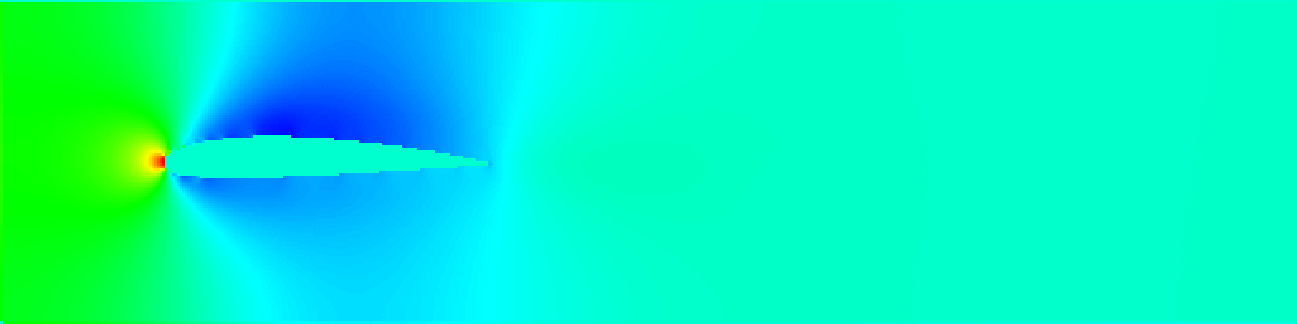
\includegraphics[width=.8\linewidth]{output/pressures}
        \caption{Pressure Scalars}
    \end{figure}
\end{frame}
\section{Performance Analysis}
\begin{frame}
    \frametitle{Execution and Test Environment}
    \begin{itemize}
        \item Exclusive node on Viking HPC cluster
        \item Dual AMD EPYC 7643 48-Core processors
            \begin{itemize}
                \item Total of 96 cores at 2.3GHz
                \item CPU has AVX2 capability for 256-bit SIMD vector registers
                \item NVIDIA H100 GPU
                \item 100Gb Intel Omni-Path node interconnect
            \end{itemize}
        \item IntelLLVM 2024 OneAPI compiler
        \item All CFD applications built to \emph{Release} mode
            \begin{itemize}
                \item Fast math optimisations
                \item Debugging symbols included
                \item Aggressive vectorisation
            \end{itemize}
        \item All executions run for two seconds of simulation time in a
            $4\text{m} \times 1\text{m}$ space with a dynamic time-step $\delta
            t$.
        \item Serialisation disabled during gathering of performance counters
    \end{itemize}
\end{frame}
\begin{frame}
    \frametitle{Serial Performance ($256\text{px} \times 64\text{px}$)}
    \centering
    \begin{tabular}{lll}
        \textbf{Section} & \textbf{Time (s)} & \textbf{Time (\%)} \\
        \toprule
        Total & 3.98 & 100 \\
        \midrule
        SOR (pressure) & 3.87 & 98.2 \\
        Tentative Velocities & 0.06 & 1.5 \\
        Poisson Source & 0.02 & 0.5
    \end{tabular}
    \begin{figure}
        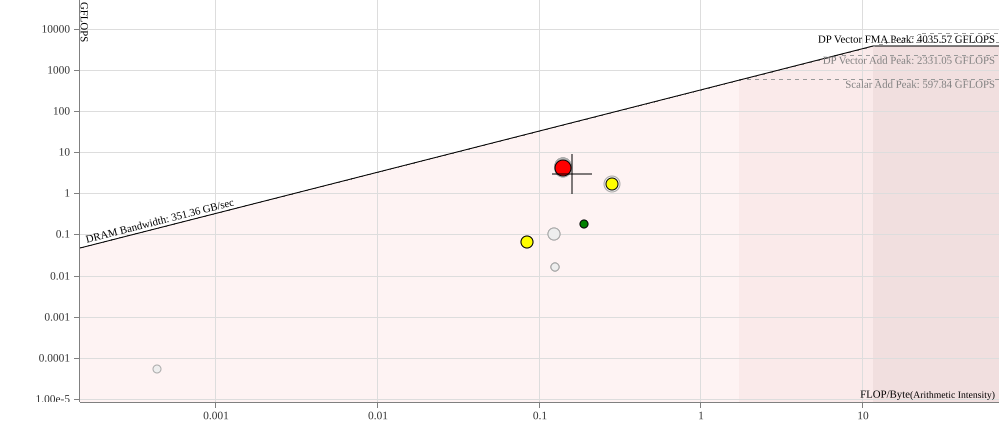
\includegraphics[width=.9\linewidth]{roofline/serial_256x64}
    \end{figure}
\end{frame}
\begin{frame}
    \frametitle{Serial Performance ($512\text{px} \times 128\text{px}$)}
    \centering
    \begin{tabular}{lll}
        \textbf{Section} & \textbf{Time (s)} & \textbf{Time (\%)} \\
        \toprule
        Total & 31.37 & 100 \\
        \midrule
        SOR (pressure) & 30.78 & 98.1 \\
        Tentative Velocities & 0.44 & 1.4 \\
        Poisson Source & 0.11 & 0.4
    \end{tabular}
    \begin{figure}
        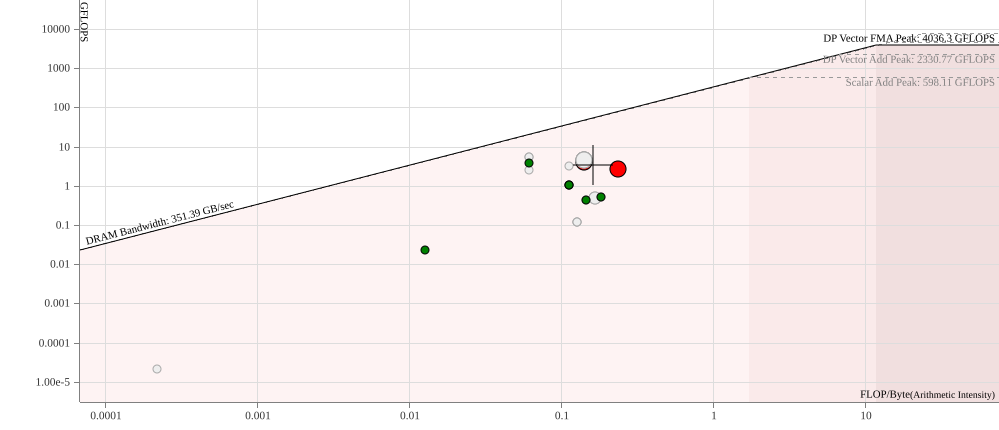
\includegraphics[width=.9\linewidth]{roofline/serial_512x128}
    \end{figure}
\end{frame}
\begin{frame}
    \frametitle{Serial Performance ($1024\text{px} \times 256\text{px}$)}
    \centering
    \begin{tabular}{lll}
        \textbf{Section} & \textbf{Time (s)} & \textbf{Time (\%)} \\
        \toprule
        Total & 382.97 & 100 \\
        \midrule
        SOR (pressure) & 375.81 & 98.1 \\
        Tentative Velocities & 5.16 & 1.3 \\
        Poisson Source & 1.08 & 0.3
    \end{tabular}
    \begin{figure}
        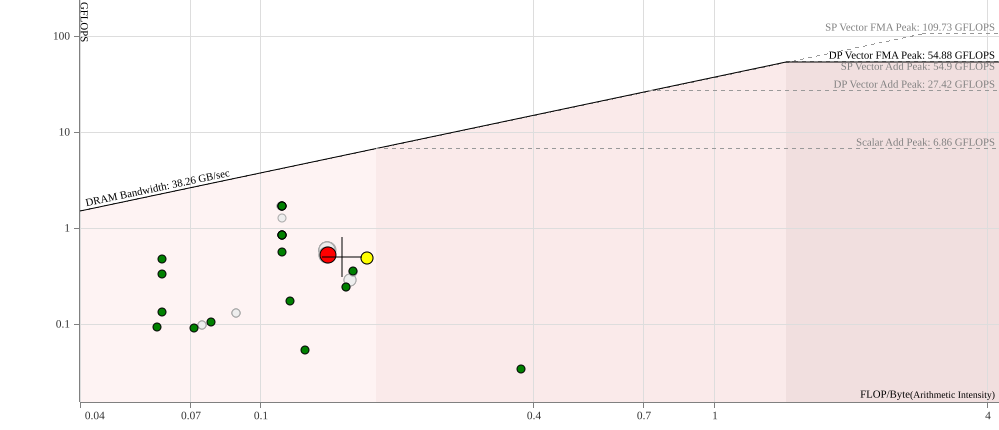
\includegraphics[width=.9\linewidth]{roofline/serial_1024x256}
    \end{figure}
\end{frame}
\begin{frame}
    \frametitle{OpenMP Performance ($256\text{px} \times 64\text{px}$)}
    \centering
    \begin{tabular}{lll}
        \textbf{Section} & \textbf{Time (s)} & \textbf{Time (\%)} \\
        \toprule
        Total & 6.8 & 100 \\
        OpenMP barriers & 2.079 & 30.57 \\
        OpenMP thread despatch & 1.85 & 27.22 \\
        \midrule
        SOR (pressure) & 1.38 & 20.29 \\
        Poisson residual & 1.09 & 16.03
    \end{tabular}
    \begin{figure}
        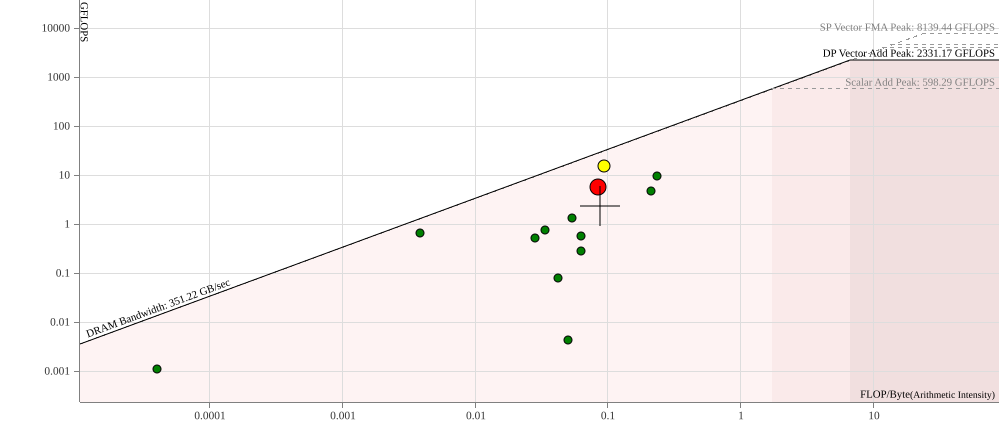
\includegraphics[width=.8\linewidth]{roofline/openmp_256x64}
    \end{figure}
\end{frame}
\begin{frame}
    \frametitle{OpenMP Performance ($512\text{px} \times 128\text{px}$)}
    \centering
    \begin{tabular}{lll}
        \textbf{Section} & \textbf{Time (s)} & \textbf{Time (\%)} \\
        \toprule
        Total & 11.65 & 100 \\
        OpenMP barriers & 2.67 & 22.89 \\
        OpenMP thread despatch & 5.69 & 48.87 \\
        \midrule
        SOR (pressure) & 1.15 & 9.87 \\
        Poisson residual & 1.57 & 13.47
    \end{tabular}
    \begin{figure}
        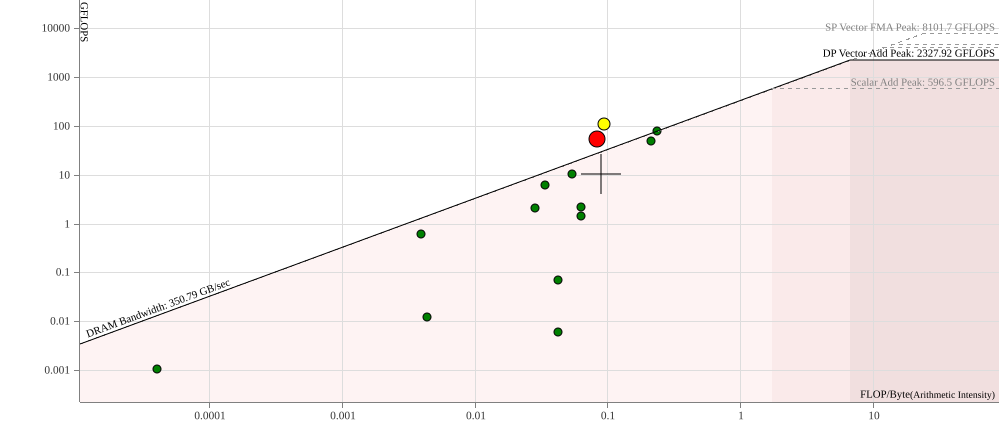
\includegraphics[width=.8\linewidth]{roofline/openmp_512x128}
    \end{figure}
\end{frame}
\begin{frame}
    \frametitle{OpenMP Performance ($1024\text{px} \times 256\text{px}$)}
    \centering
    \begin{tabular}{lll}
        \textbf{Section} & \textbf{Time (s)} & \textbf{Time (\%)} \\
        \toprule
        Total & 42.02 & 100 \\
        OpenMP barriers & 8.321 & 19.8 \\
        OpenMP thread despatch & 20.9 & 49.73 \\
        \midrule
        SOR (pressure) & 5.02 & 11.95 \\
        Poisson residual & 6.01 & 14.3
    \end{tabular}
    \begin{figure}
        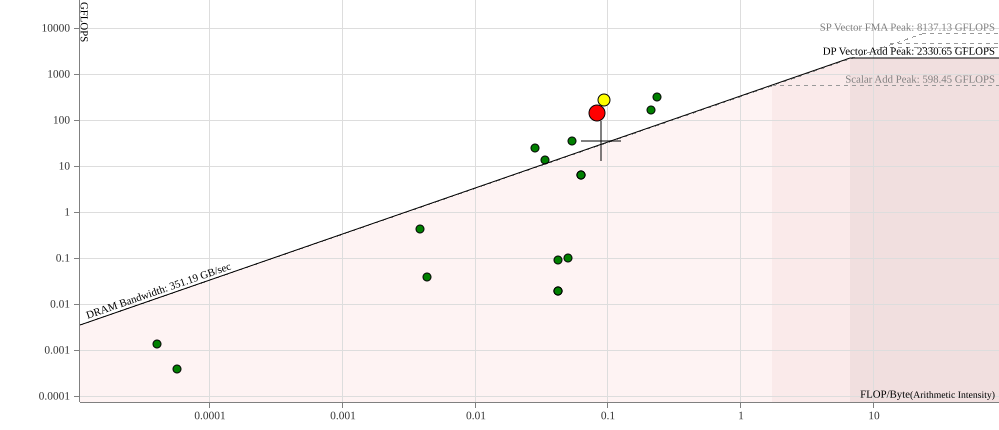
\includegraphics[width=.8\linewidth]{roofline/openmp_1024x256}
    \end{figure}
\end{frame}
\begin{frame}
    \frametitle{MPI Performance ($256\text{px} \times 64\text{px}$)}
    \centering
    \begin{tabular}{lll}
        \textbf{Section} & \textbf{Time (s)} & \textbf{Time (\%)} \\
        \toprule
        Total & 1.1 & 100 \\
        MPI startup and teardown & 0.68 & 60.1 \\
        \midrule
        SOR (pressure) & 0.03 & 2.7 \\
        Halo exchanges & 0.14 & 12.4 \\
        Reductions & 0.18 & 15.9
    \end{tabular}
    \begin{figure}
        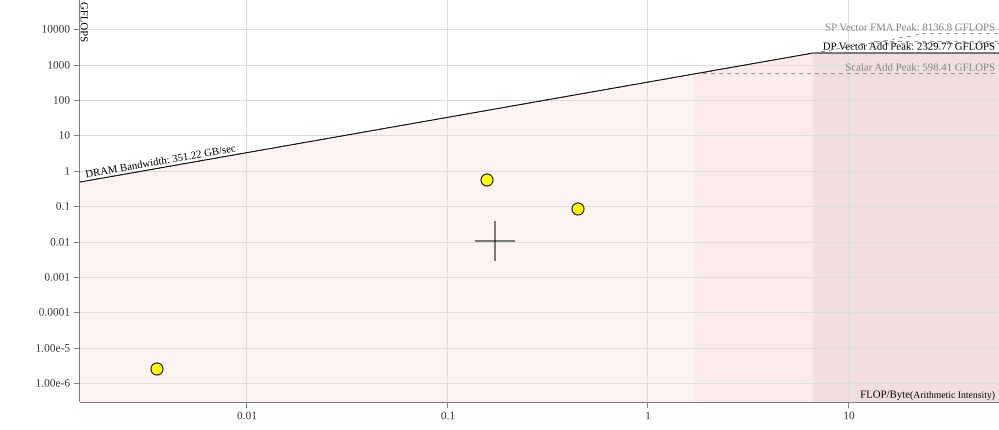
\includegraphics[width=.8\linewidth]{roofline/mpi_256x64}
    \end{figure}
\end{frame}
\begin{frame}
    \frametitle{MPI Performance ($512\text{px} \times 128\text{px}$)}
    \centering
    \begin{tabular}{lll}
        \textbf{Section} & \textbf{Time (s)} & \textbf{Time (\%)} \\
        \toprule
        Total & 2.51 & 100 \\
        MPI startup and teardown & 0.63 & 24.9 \\
        \midrule
        SOR (pressure) & 0.27 & 10.7 \\
        Halo exchanges & 0.52 & 20.6 \\
        Reductions & 1.03 & 40.3
    \end{tabular}
    \begin{figure}
        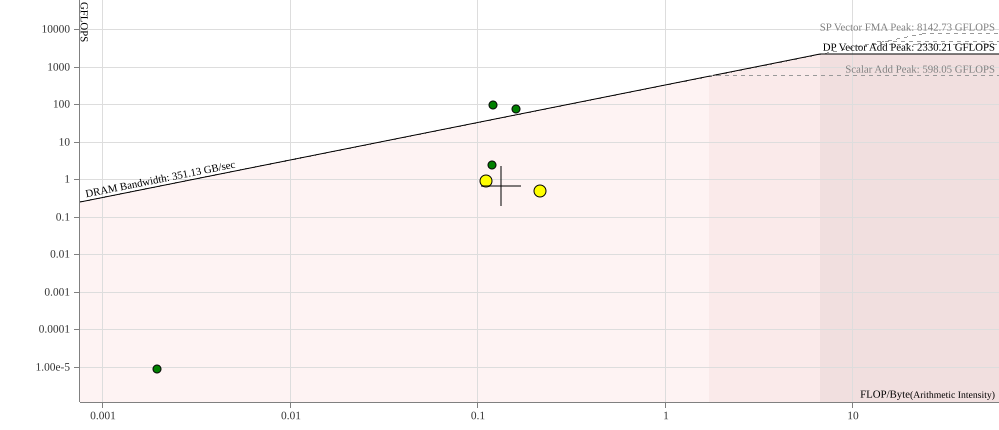
\includegraphics[width=.8\linewidth]{roofline/mpi_512x128}
    \end{figure}
\end{frame}
\begin{frame}
    \frametitle{MPI Performance ($1024\text{px} \times 256\text{px}$)}
    \centering
    \begin{tabular}{lll}
        \textbf{Section} & \textbf{Time (s)} & \textbf{Time (\%)} \\
        \toprule
        Total & 8.95 & 100 \\
        MPI startup and teardown & 0.7 & 7.8 \\
        \midrule
        SOR (pressure) & 2.68 & 29.8 \\
        Halo exchanges & 1.33 & 14.8 \\
        Reductions & 2.01 & 22.3
    \end{tabular}
    \begin{figure}
        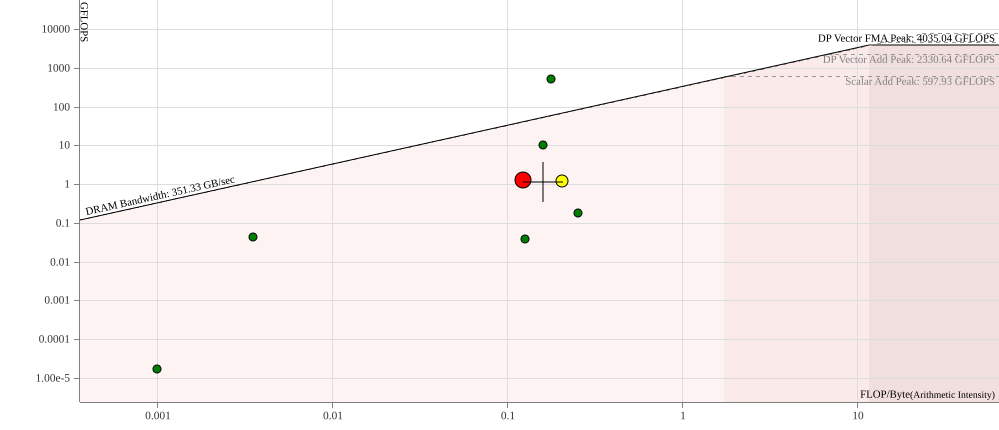
\includegraphics[width=.8\linewidth]{roofline/mpi_1024x256}
    \end{figure}
\end{frame}
\begin{frame}
    \frametitle{CUDA Performance ($256\text{px} \times 64\text{px}$)}
    \centering
    \begin{tabular}{lll}
        \textbf{Section} & \textbf{Time (s)} & \textbf{Time (\%)} \\
        \toprule
        Total & & 100 \\
        \midrule
        SOR (pressure) & & \\
        Tentative Velocities & & \\
        Poisson Source & & 
    \end{tabular}
    %\begin{figure}
    %    \includegraphics[width=.9\linewidth]{roofline/cuda_256x64}
    %\end{figure}
\end{frame}
\begin{frame}
    \frametitle{CUDA Performance ($512\text{px} \times 128\text{px}$)}
    \centering
    \begin{tabular}{lll}
        \textbf{Section} & \textbf{Time (s)} & \textbf{Time (\%)} \\
        \toprule
        Total & & 100 \\
        \midrule
        SOR (pressure) & & \\
        Tentative Velocities & & \\
        Poisson Source & & 
    \end{tabular}
    %\begin{figure}
    %    \includegraphics[width=.9\linewidth]{roofline/cuda_512x128}
    %\end{figure}
\end{frame}
\begin{frame}
    \frametitle{CUDA Performance ($1024\text{px} \times 256\text{px}$)}
    \centering
    \begin{tabular}{lll}
        \textbf{Section} & \textbf{Time (s)} & \textbf{Time (\%)} \\
        \toprule
        Total & & 100 \\
        \midrule
        SOR (pressure) & & \\
        Tentative Velocities & & \\
        Poisson Source & & 
    \end{tabular}
    %\begin{figure}
    %    \includegraphics[width=.9\linewidth]{roofline/cuda_1024x256}
    %\end{figure}
\end{frame}
\section{Performance Comparison and Discussion}
\begin{frame}
    \frametitle{Performance Comparison (1)}
    \begin{center}
        \begin{figure}
            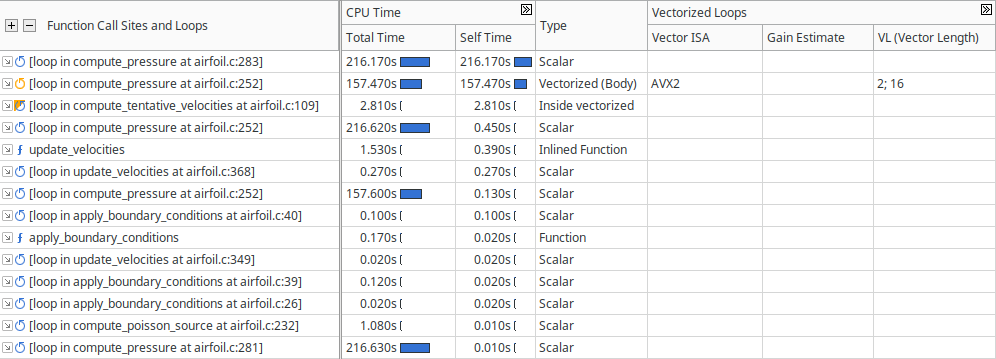
\includegraphics[width=.65\linewidth]{intel-tools/scalar-advisor}
            \caption{Scalar SOR implementation}
        \end{figure}
        \begin{figure}
            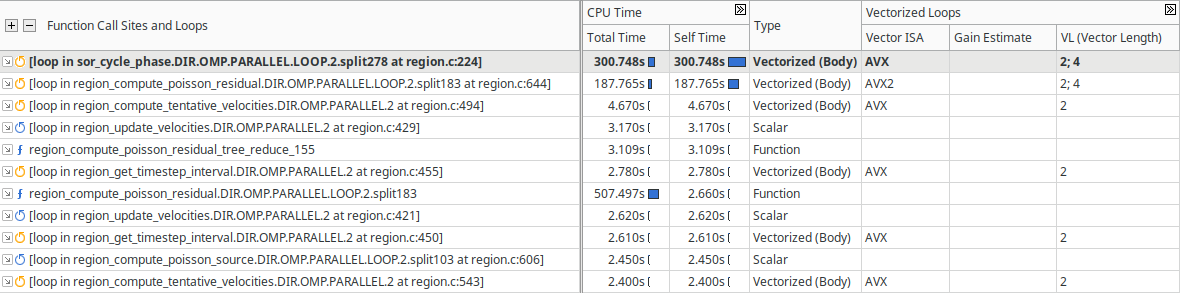
\includegraphics[width=.65\linewidth]{intel-tools/avx-advisor}
            \caption{Vectorised SOR implementation}
        \end{figure}
    \end{center}
\end{frame}
\begin{frame}
    \frametitle{Performance Comparison (2)}
    \begin{center}
        \begin{tikzpicture}
        \begin{axis}[
            ybar=4pt,
            ylabel={Wall clock runtime (s)},
            xlabel={Problem space size (px)},
            symbolic x coords={256$\times$64,512$\times$128,1024$\times$256},
            xtick=data,
            ymin=0,
            legend cell align=left,
            legend pos=north west,
            enlarge x limits=0.5,
            height=0.8\textheight,
            width=0.9\textwidth
        ]

        % Serial
        \addplot[fill=seriallegend] coordinates {
            (256$\times$64, 3.98)
            (512$\times$128, 31.37)
            (1024$\times$256, 382.97)
        };

        % OpenMP
        \addplot[fill=openmplegend] coordinates {
            (256$\times$64, 6.8)
            (512$\times$128, 11.65)
            (1024$\times$256, 42.02)
        };

        % MPI
        \addplot[fill=mpilegend] coordinates {
            (256$\times$64, 1.1)
            (512$\times$128, 2.51)
            (1024$\times$256, 8.95)
        };

        % CUDA
        \addplot[fill=cudalegend] coordinates {
            (256$\times$64, 0)
            (512$\times$128, 0)
            (1024$\times$256, 0)
        };

        \legend{Serial, OpenMP, MPI, CUDA}

        \end{axis}
        \end{tikzpicture}
    \end{center}
\end{frame}
\begin{frame}
    \frametitle{Performance Comparison (3)}
    \begin{center}
        \begin{tikzpicture}
        \begin{axis}[
            ybar=4pt,
            ylabel={Wall clock runtime (s)},
            xlabel={Problem space size (px)},
            symbolic x coords={256$\times$64,512$\times$128,1024$\times$256},
            xtick=data,
            ymin=0,
            legend cell align=left,
            legend pos=north west,
            enlarge x limits=0.5,
            height=0.8\textheight,
            width=0.9\textwidth
        ]

        % OpenMP
        \addplot[fill=openmplegend] coordinates {
            (256$\times$64, 6.8)
            (512$\times$128, 11.65)
            (1024$\times$256, 42.02)
        };

        % MPI
        \addplot[fill=mpilegend] coordinates {
            (256$\times$64, 1.1)
            (512$\times$128, 2.51)
            (1024$\times$256, 8.95)
        };

        % CUDA
        \addplot[fill=cudalegend] coordinates {
            (256$\times$64, 0)
            (512$\times$128, 0)
            (1024$\times$256, 0)
        };

        \legend{OpenMP, MPI, CUDA}

        \end{axis}
        \end{tikzpicture}
    \end{center}
\end{frame}
\begin{frame}
    \frametitle{Solution Comparison}
    \begin{itemize}
        \item All solutions engineered to follow object-oriented principles
            \begin{itemize}
                \item Faster to organise code in CUDA due to features inherited
                    from C++11, 14, and 17.
                \item OpenMP approx. 1082 LOC; MPI 1940; CUDA 1333.
            \end{itemize}
        \item OpenMP and MPI solutions highly portable at runtime; CUDA
            vendor-locked to proprietary NVIDIA technology.
        \item All solutions can be subject to dynamic analysis for profiling and
            correctness checks (e.g. Valgrind, ASan, \texttt{cuda-memchk}).
        \item MPI and CUDA substantially more effort to interactively debug due
            to distributed topology.
        \item Build process and remote workflows homogenised by modern tools
            \begin{itemize}
                \item CMake
                \item CLion
                \item LLDB remote debugging
                \item OneAPI userland tools
            \end{itemize}
    \end{itemize}
\end{frame}
\section{}
\begin{frame}
    \frametitle{Thank you for listening}
\end{frame}
\end{document}

